% Copyright 2020 Glen Newton
% License: Creative Commons Attribution-ShareAlike 4.0 International License https://creativecommons.org/licenses/by-sa/4.0/legalcode
%\documentclass[a0paper,10pt]{article}
\documentclass[12pt]{article}


\usepackage{tikz}
\usepackage[margin=6mm]{geometry}

\usepackage[extreme]{savetrees}
\usepackage{microtype}
\usepackage[hidelinks]{hyperref}
\usetikzlibrary{mindmap,positioning}

%\usepackage{atbegshi}% http://ctan.org/pkg/atbegshi
%\AtBeginDocument{\AtBeginShipoutNext{\AtBeginShipoutDiscard}}


% from: https://tex.stackexchange.com/questions/250150/formatting-mindmap-in-tikz
\hypersetup{
  colorlinks=false
}

\definecolor{myb}{rgb}{0, 0, 0.6}

% from: https://tex.stackexchange.com/questions/107057/adjusting-font-size-with-tikz-picture

\begin{document}

\sffamily
\pagestyle{empty}

{\centering
  \noindent
  \makebox[0pt]{%
    \resizebox{\columnwidth}{!}
              {
                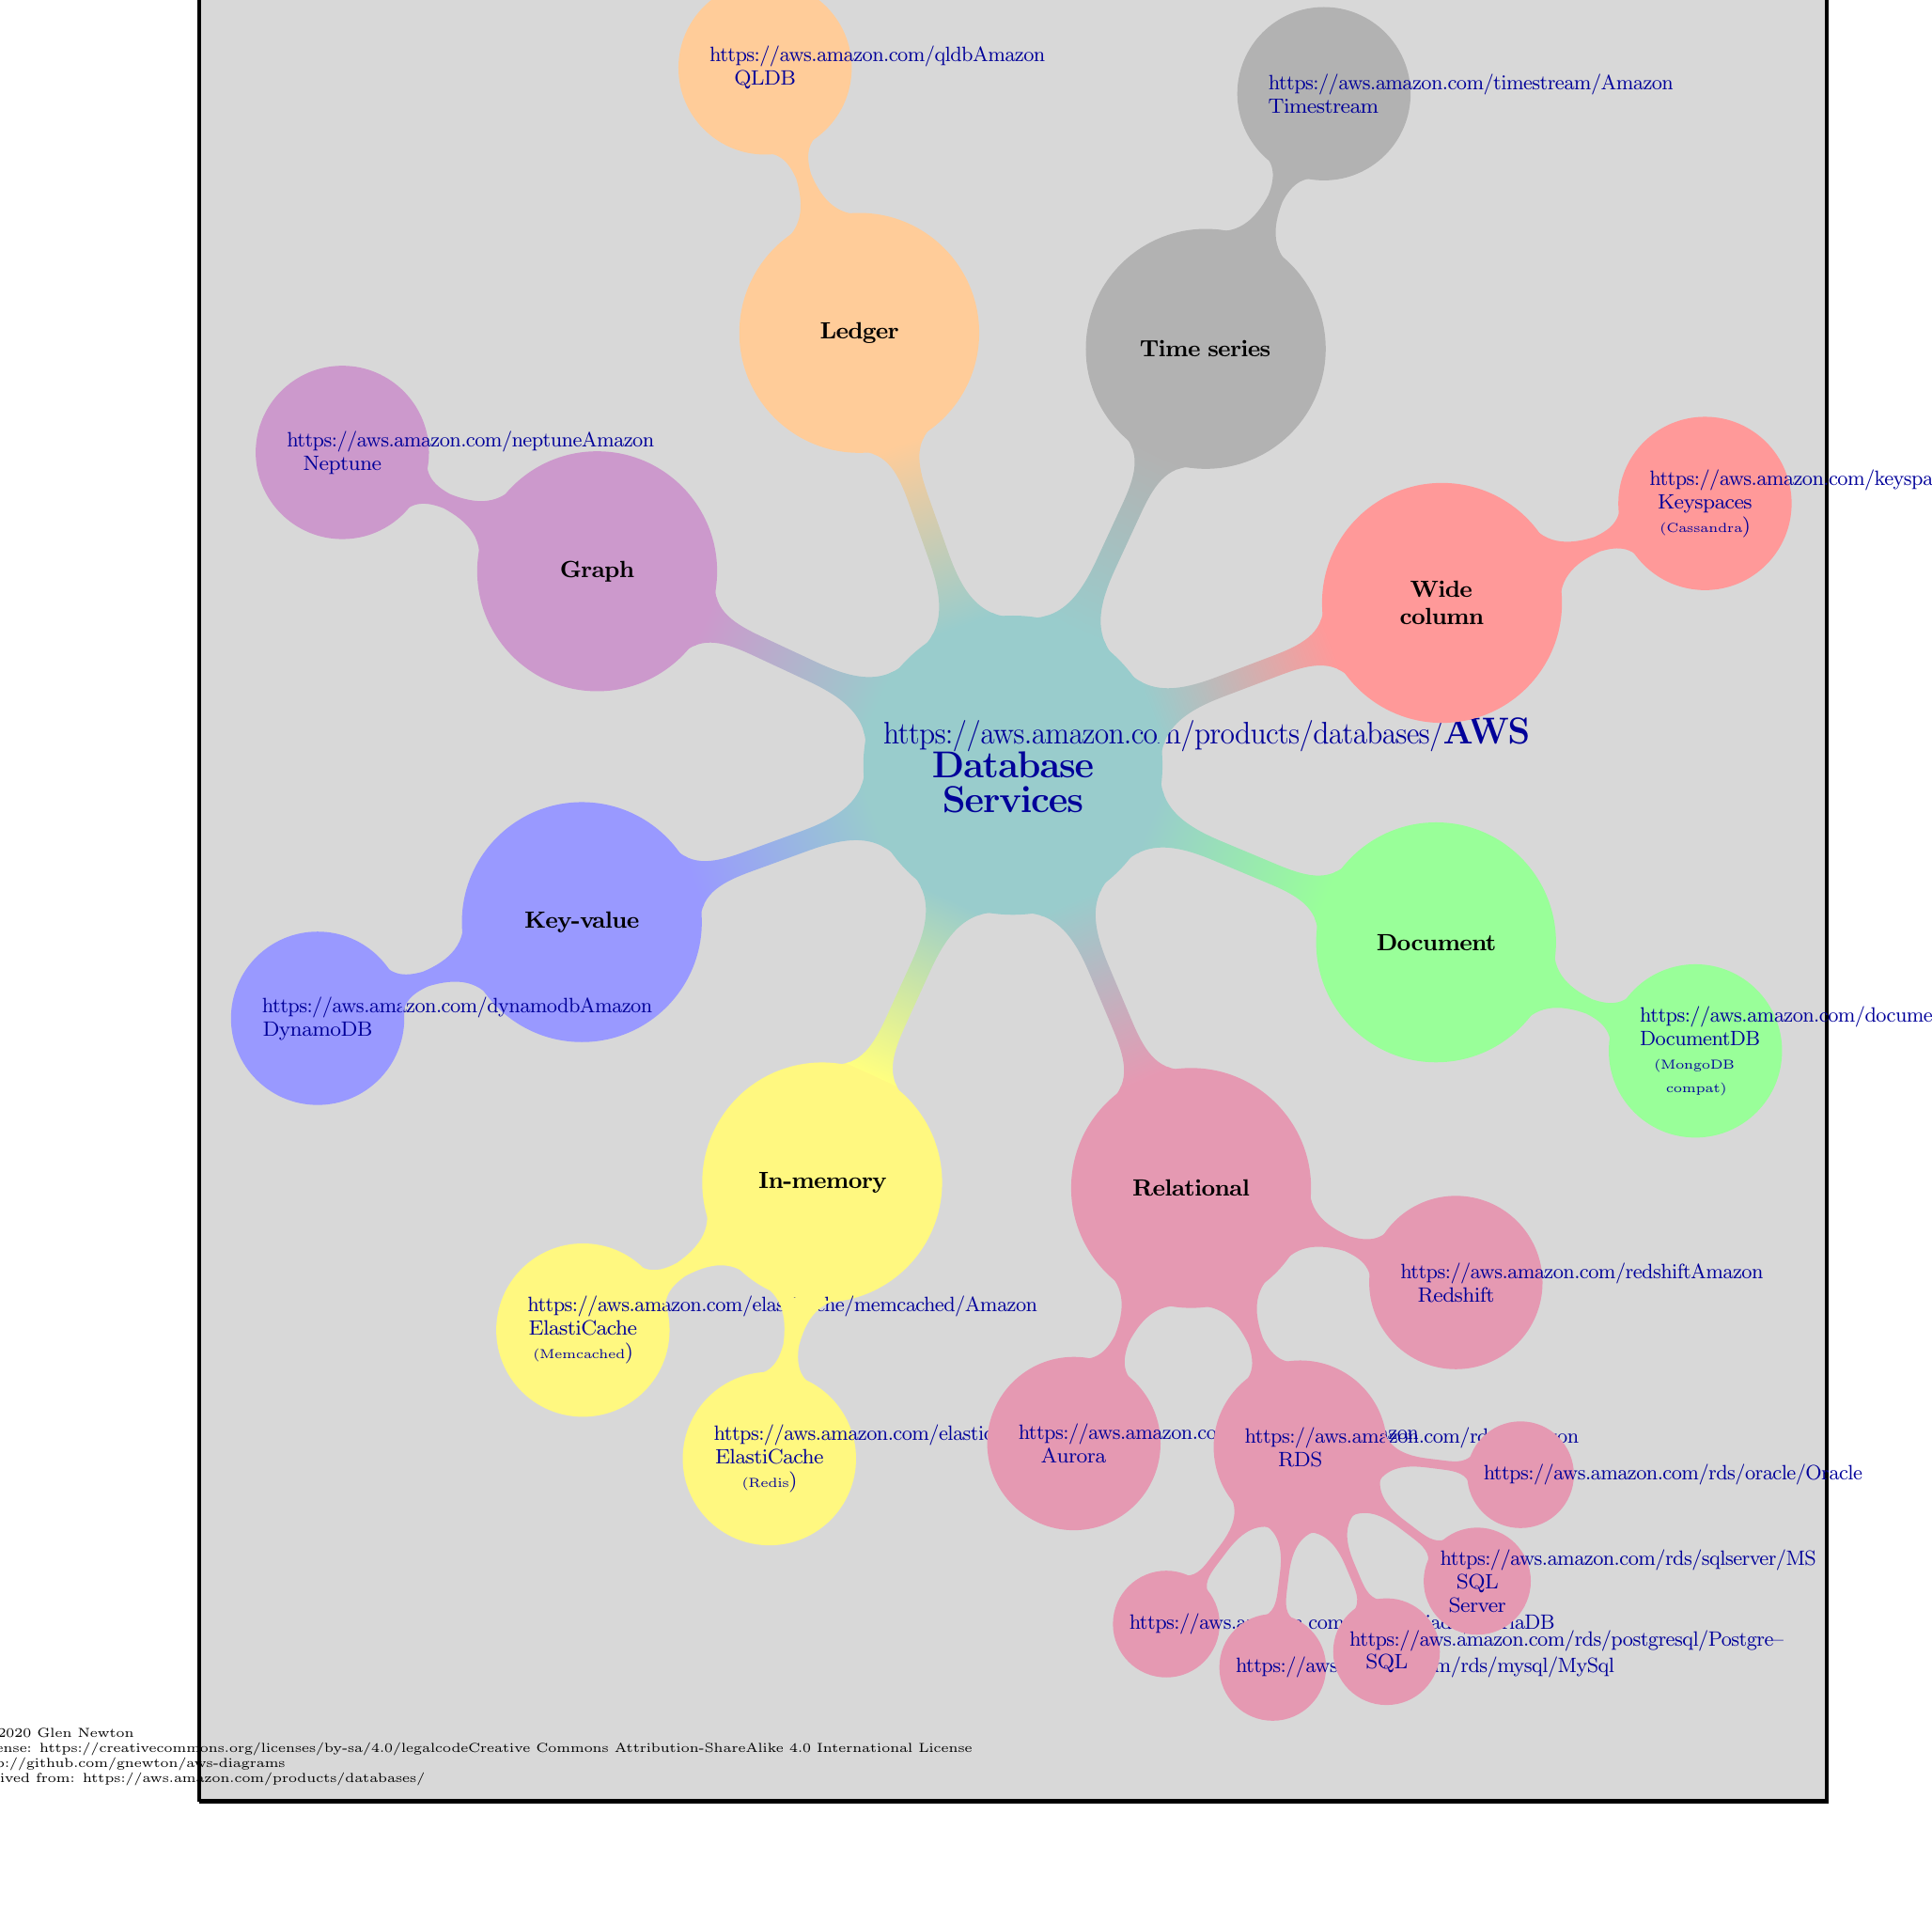
\begin{tikzpicture}
                  \begin{scope}
                    \draw [ultra thick, fill=gray!60, fill opacity=0.5] (-11,-14) -- (11,-14) -- (11,11) -- (-11,11) -- (-11,-14);
                  \end{scope}
                  \begin{scope}
                    [mindmap,
                      grow cyclic,
                      every node/.style=concept,
                      concept color=teal!40,
                      level 1/.append style={sibling angle=360/7, level distance=6.2cm,minimum size=3.2cm},
                      level 2/.append style={sibling angle=37.5, level distance=3.8cm,minimum size=2.3cm},
                      level 3/.append style={level distance=3cm,minimum size=1.4cm,font=\footnotesize},
                    ]
                    \node [root concept] {\color{myb} \href{https://aws.amazon.com/products/databases/}{\Large \bfseries AWS Database Services}}
                    child [concept color=blue!40, rotate=20]{
                      node[concept] {\bfseries Key-value}
                      child { node[concept] {\color{myb} \href{https://aws.amazon.com/dynamodb}{Amazon\\ DynamoDB}} }
                    }
                    child [concept color=yellow!50, rotate=14]{
                      node   {\bfseries In-memory}%[clockwise from=45, level distance=8cm]
                      child [rotate=-15]{ node[concept,alias=foo] {\color{myb} \href{https://aws.amazon.com/elasticache/memcached/}{Amazon\\ ElastiCache\\ {\tiny (Memcached})}} }
                      child [rotate=-5]{ node[concept] {\color{myb} \href{https://aws.amazon.com/elasticache/redis}{Amazon\\ ElastiCache}\\ {\tiny (Redis})} }
                    }
                    child [concept color=purple!40, rotate=10]{
                      node    {\bfseries Relational}
                      child [rotate=-10]{ node    {\color{myb} \href{https://aws.amazon.com/rds/aurora/}{Amazon Aurora}}}
                      child { node    {\color{myb} \href{https://aws.amazon.com/rds/}{Amazon RDS}}
                        child { node[concept] {\color{myb} \href{https://aws.amazon.com/rds/mariadb/}{MariaDB}} }
                        child { node[concept] {\color{myb} \href{https://aws.amazon.com/rds/mysql/}{MySql}} }
                        child { node[concept] {\color{myb} \href{https://aws.amazon.com/rds/postgresql/}{Postgre-- SQL} }}
                        child { node[concept] {\color{myb} \href{https://aws.amazon.com/rds/sqlserver/}{MS SQL Server} }}
                        child { node[concept] {\color{myb} \href{https://aws.amazon.com/rds/oracle/}{Oracle} }}
                      }
                      child [rotate=10] { node    {\color{myb} \href{https://aws.amazon.com/redshift}{Amazon Redshift}} }
                    }
                    child [concept color=green!40, rotate=3]{
                      node     {\bfseries Document}
                      child { node    {\color{myb} \href{https://aws.amazon.com/documentdb}{Amazon\\ DocumentDB\\{\tiny (MongoDB compat)}}} }
                    }
                    child [concept color=red!40, rotate=-5]{node  {\bfseries Wide column}
                      child { node[concept] {\color{myb}  \href{https://aws.amazon.com/keyspaces/}{Amazon Keyspaces\\{\tiny (Cassandra})}} }
                    }
                    child [concept color=gray!60, rotate=-12]{node  {\bfseries Time series}
                      child { node[concept] {\color{myb} \href{https://aws.amazon.com/timestream/}{Amazon Timestream}} }
                    }
                    child [concept color=orange!40, rotate=-19] {node {\bfseries Ledger}
                      child { node {\color{myb} \href{https://aws.amazon.com/qldb}{Amazon QLDB}} }
                    }
                    child [concept color=violet!40, rotate=-25] {node {\bfseries Graph}
                      child { node {\color{myb} \href{https://aws.amazon.com/neptune}{Amazon Neptune}} }
                    };
                  \end{scope}
                  \node[xshift=-7.3cm,yshift=-13.3cm](foox) {
                    %                  Copyright 2020 Glen Newton
                                      \tiny
                  \begin{tabular}{l}
                  \\
                    \copyright \ 2020 Glen Newton\\
                    License: \href{https://creativecommons.org/licenses/by-sa/4.0/legalcode}{Creative Commons Attribution-ShareAlike 4.0 International License}\\
                    \url{http://github.com/gnewton/aws-diagrams} \\
                    Derived from: \url{https://aws.amazon.com/products/databases/}
                  \end{tabular}

                  };
  \end{tikzpicture}}}\par}


\end{document}
